\chapter{Diagrames}
\label{appendix:diagrams}
En aquest ap�ndix es mostren alguns diagrames que poden ajudar a entendre una mica millor l'aplicaci�. Creiem que cada diagrama �s autoexplicatiu nom�s s'acompanyen d'una petita descripci� als peus de cadascun d'ells.

\begin{figure}[H]
\begin{center}
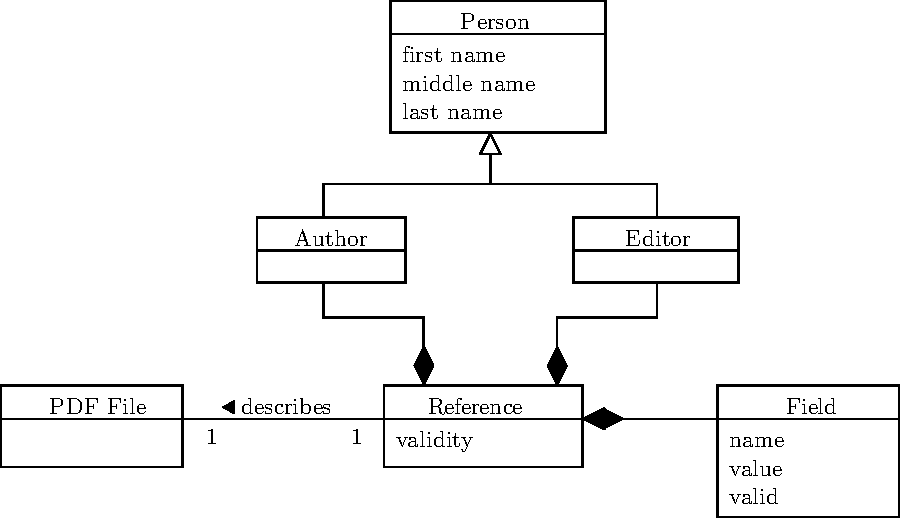
\includegraphics[width=0.7\textwidth]{figures/diagrams:references-domain-model.pdf}
\caption{Model de domini respecte a refer�ncies}
\label{fig:diagrams:references-domain-model}
\end{center}
\end{figure}


\begin{figure}[H]
\begin{center}
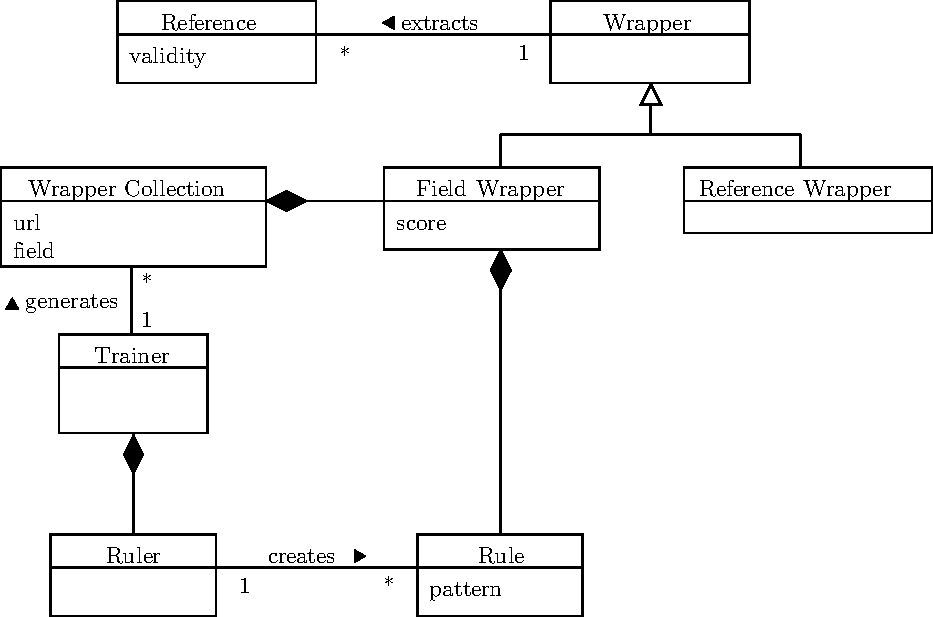
\includegraphics[width=0.7\textwidth]{figures/diagrams:wrappers-domain-model.pdf}
\caption{Model de domini dels \textit{wrappers}}
\label{fig:diagrams:wrappers-domain-model}
\end{center}
\end{figure}

\begin{figure}[H]
\begin{center}
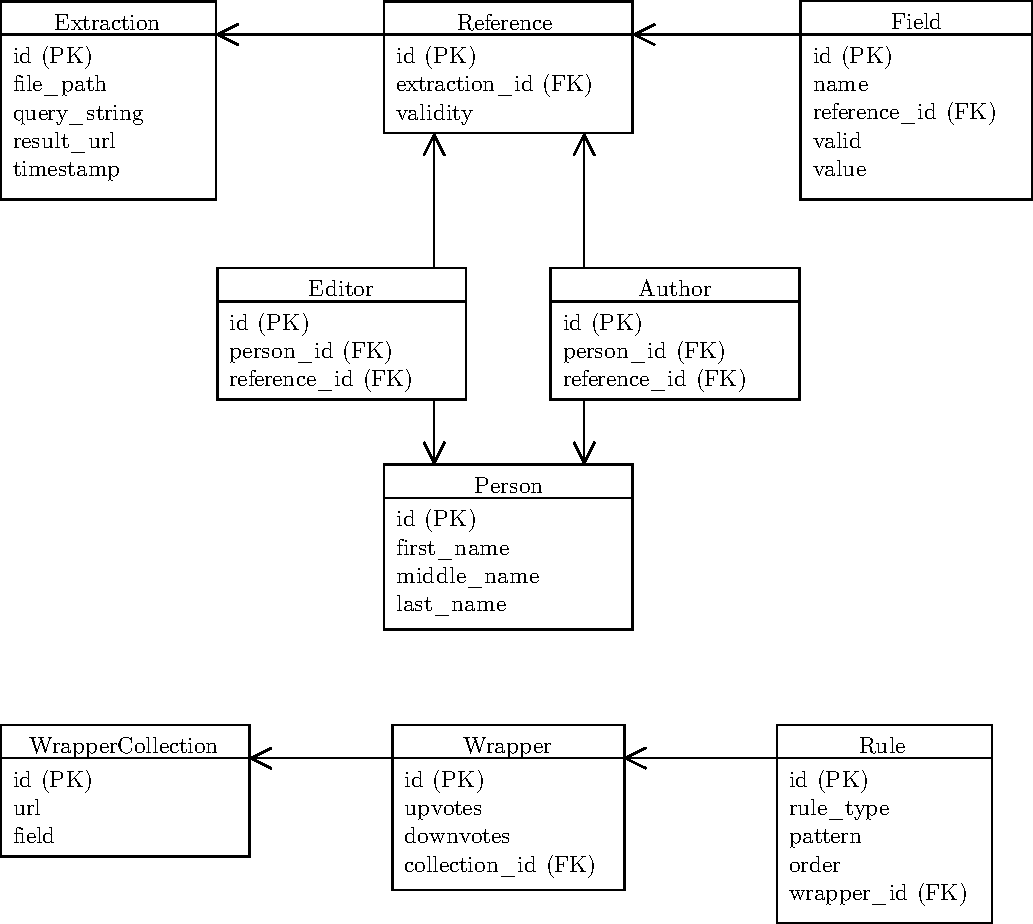
\includegraphics[width=0.8\textwidth]{figures/diagrams:database-diagram.pdf}
\caption{Estructura de la base de dades}
\label{fig:diagrams:database-diagram}
\end{center}
\end{figure}


\begin{figure}[ht]
\begin{center}
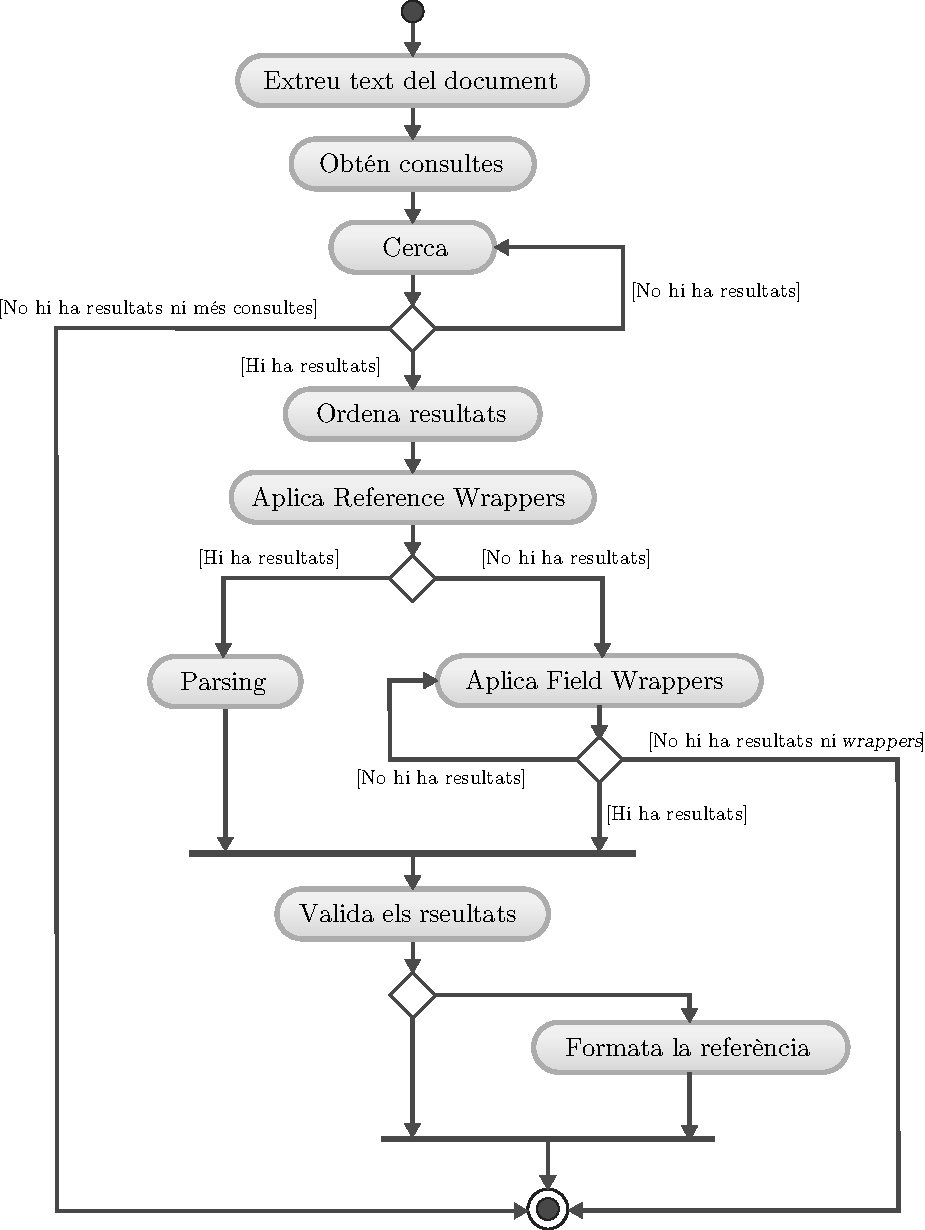
\includegraphics[width=0.95\textwidth]{figures/diagrams:extraction-activity.pdf}
\caption{Diagrama d'activitat per a l'extracci� de refer�ncies}
\label{fig:diagrams:extraction-activity}
\end{center}
\end{figure}

\clearpage




